\documentclass[border=10pt]{standalone}
\usepackage{tikz}\usepackage{amsmath}\usetikzlibrary{arrows.meta}
\begin{document}
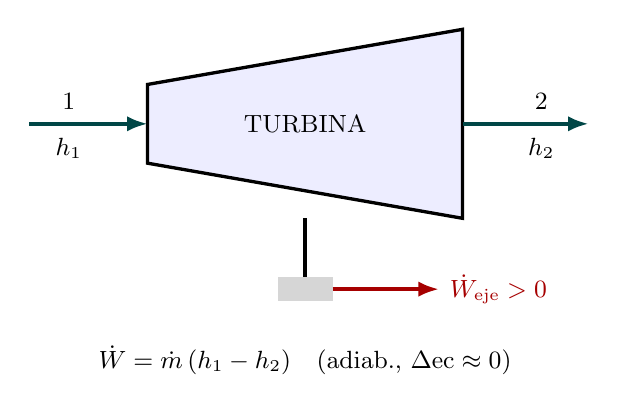
\begin{tikzpicture}[line width=1pt,>={Latex[length=2.6mm]}]
  \fill[blue!7] (0,1)--(0,2)--(4,2.7)--(4,0.3)--cycle;
  \draw[line width=1.2pt] (0,1)--(0,2)--(4,2.7)--(4,0.3)--cycle;
  \node at (2,1.5){\small TURBINA};
  \draw[->,teal!55!black,line width=1.3pt] (-1.5,1.5)--(0,1.5);
  \node[above] at (-1.0,1.55){\small $1$}; \node[below] at (-1.0,1.45){\small $h_1$};
  \draw[->,teal!55!black,line width=1.3pt] (4,1.5)--(5.6,1.5);
  \node[above] at (5.0,1.55){\small $2$}; \node[below] at (5.0,1.45){\small $h_2$};
  \draw[line width=1.3pt] (2,0.3)--(2,-0.45);
  \fill[black!16] (1.65,-0.45) rectangle (2.35,-0.75);
  \draw[->,red!65!black,line width=1.3pt] (2.35,-0.6)--(3.7,-0.6) node[right]{\small $\dot W_{\text{eje}}>0$};
  \node at (2,-1.5){\small $\dot W = \dot m\,(h_1-h_2)$\quad (adiab., $\Delta\mathrm{ec}\approx0$)};
\end{tikzpicture}
\end{document}
